\documentclass{article}

\usepackage{amsmath, amsthm, amssymb, amsfonts}
\usepackage{thmtools}
\usepackage{graphicx}
\usepackage{setspace}
\usepackage{geometry}
\usepackage{float}
\usepackage{hyperref}
\usepackage[utf8]{inputenc}
\usepackage[english]{babel}
\usepackage{framed}
\usepackage[dvipsnames]{xcolor}
\usepackage{tcolorbox}
\usepackage{fancyhdr}

\colorlet{LightGray}{White!90!Periwinkle}
\colorlet{LightOrange}{Orange!15}
\colorlet{LightGreen}{Green!15}
\pagestyle{fancy}
\fancyhf{} % Pulisce l'header e il footer predefiniti
\renewcommand{\headrulewidth}{0pt} % Opzionale: rimuove la linea orizzontale dall'header
\fancyhead[C]{\textbf{MLPR Project:\\ Fingerprint spoofing detection}} % Titolo centrato nell'header
\fancyfoot[C]{\thepage}
\newcommand{\HRule}[1]{\rule{\linewidth}{#1}}

\declaretheoremstyle[name=Theorem,]{thmsty}
\declaretheorem[style=thmsty,numberwithin=section]{theorem}
\tcolorboxenvironment{theorem}{colback=LightGray}


\declaretheoremstyle[name=Proposition,]{prosty}
\declaretheorem[style=prosty,numberlike=theorem]{proposition}
\tcolorboxenvironment{proposition}{colback=LightOrange}

\declaretheoremstyle[name=Principle,]{prcpsty}
\declaretheorem[style=prcpsty,numberlike=theorem]{principle}
\tcolorboxenvironment{principle}{colback=LightGreen}

\setstretch{1.2}
\geometry{
    textheight=9in,
    textwidth=5.5in,
    top=1in,
    headheight=12pt,
    headsep=25pt,
    footskip=30pt
}

% ------------------------------------------------------------------------------

\begin{document}

% ------------------------------------------------------------------------------
% Cover Page and ToC
% ------------------------------------------------------------------------------

\title{ \normalsize \textsc{}
		\\ [2.0cm]
		\HRule{1.5pt} \\
		\LARGE \textbf{\uppercase{Report Machine Learning and pattern recognition}
		\HRule{2.0pt} \\ [0.6cm] \LARGE{Fingerprint spoofing detection} \vspace*{10\baselineskip}}
		}
\date{}
\author{\textbf{Alessia Intini} \\ 
		s309895 \\
		Politecnico di Torino \\
		2023/24}

\maketitle
\newpage

\tableofcontents
\newpage

% ------------------------------------------------------------------------------
\noindent\textbf{The goal of project is to perform a binary classification on fingerprint spoofing detection, that is to identify genuine vs counterfeit fingerprint images. The dataset consists of labeled samples corresponding to the genuine (True, label 1) class and the fake (False, label 0) class, the data is 6-dimensional.}
\section{Dataset Analysis}
\subsection{Training and evaluation sets}
The datasets provided contain 6000 samples; the first 6 values in each row represent the features, while the last value is the label. Specifically they are: 
\begin{itemize}
    \item Training Set: 2990 samples beloging to the Fake class (label 0) and 3010 samples belonging to the Genuine class (label 1)
    \item Evaluation Set: 3010 samples beloging to the Fake class (label 0) and 2990 samples belonging to the Genuine class (label 1)
\end{itemize}
We will use the Training Set to perform all the analysis, during this phase the dataset is divided to use about 60\% of it as the training dataset and the remaining 40\% for validation. 
After this step, the most promising models were chosen and the evaluation dataset was used to evaluate them and make the final considerations.
\subsection{Features analysis}
We can start to analize all features, here is the graph of each feature, through these histograms it is shown how each feature is distributed:\\
\begin{figure}[ht]

        \centering
        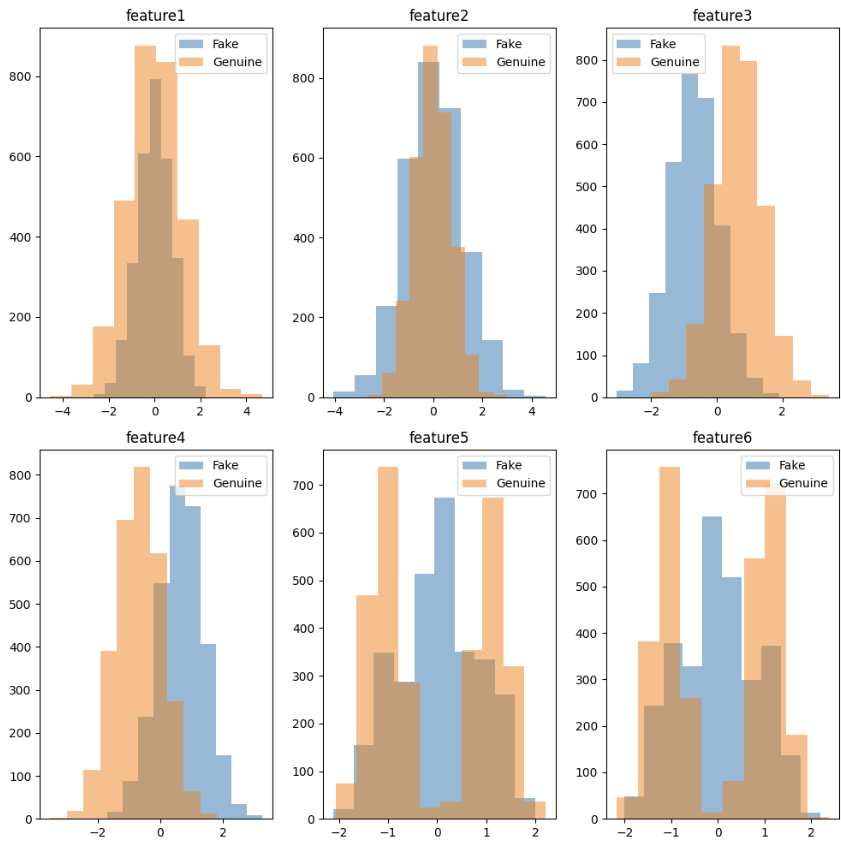
\includegraphics[width=0.5\textwidth]{./img/AllFeatures.png}
        \caption{All features}
        \label{fig:AllFeatures}
\end{figure}  
\\
By plotting a histogram for each feature, separately for the Fake and Genuine classes, it is possible to show whether the samples follow a Gaussian distribution and to what extent. 
Thus, we can say that some features follow a Gaussian distribution. Furthermore, it can be seen that features 4 and 5 may be the most discriminating features based on their ability to separate the data of the two classes.\\
\begin{figure}[ht]
    \begin{minipage}[b]{0.45\textwidth}
        \centering
        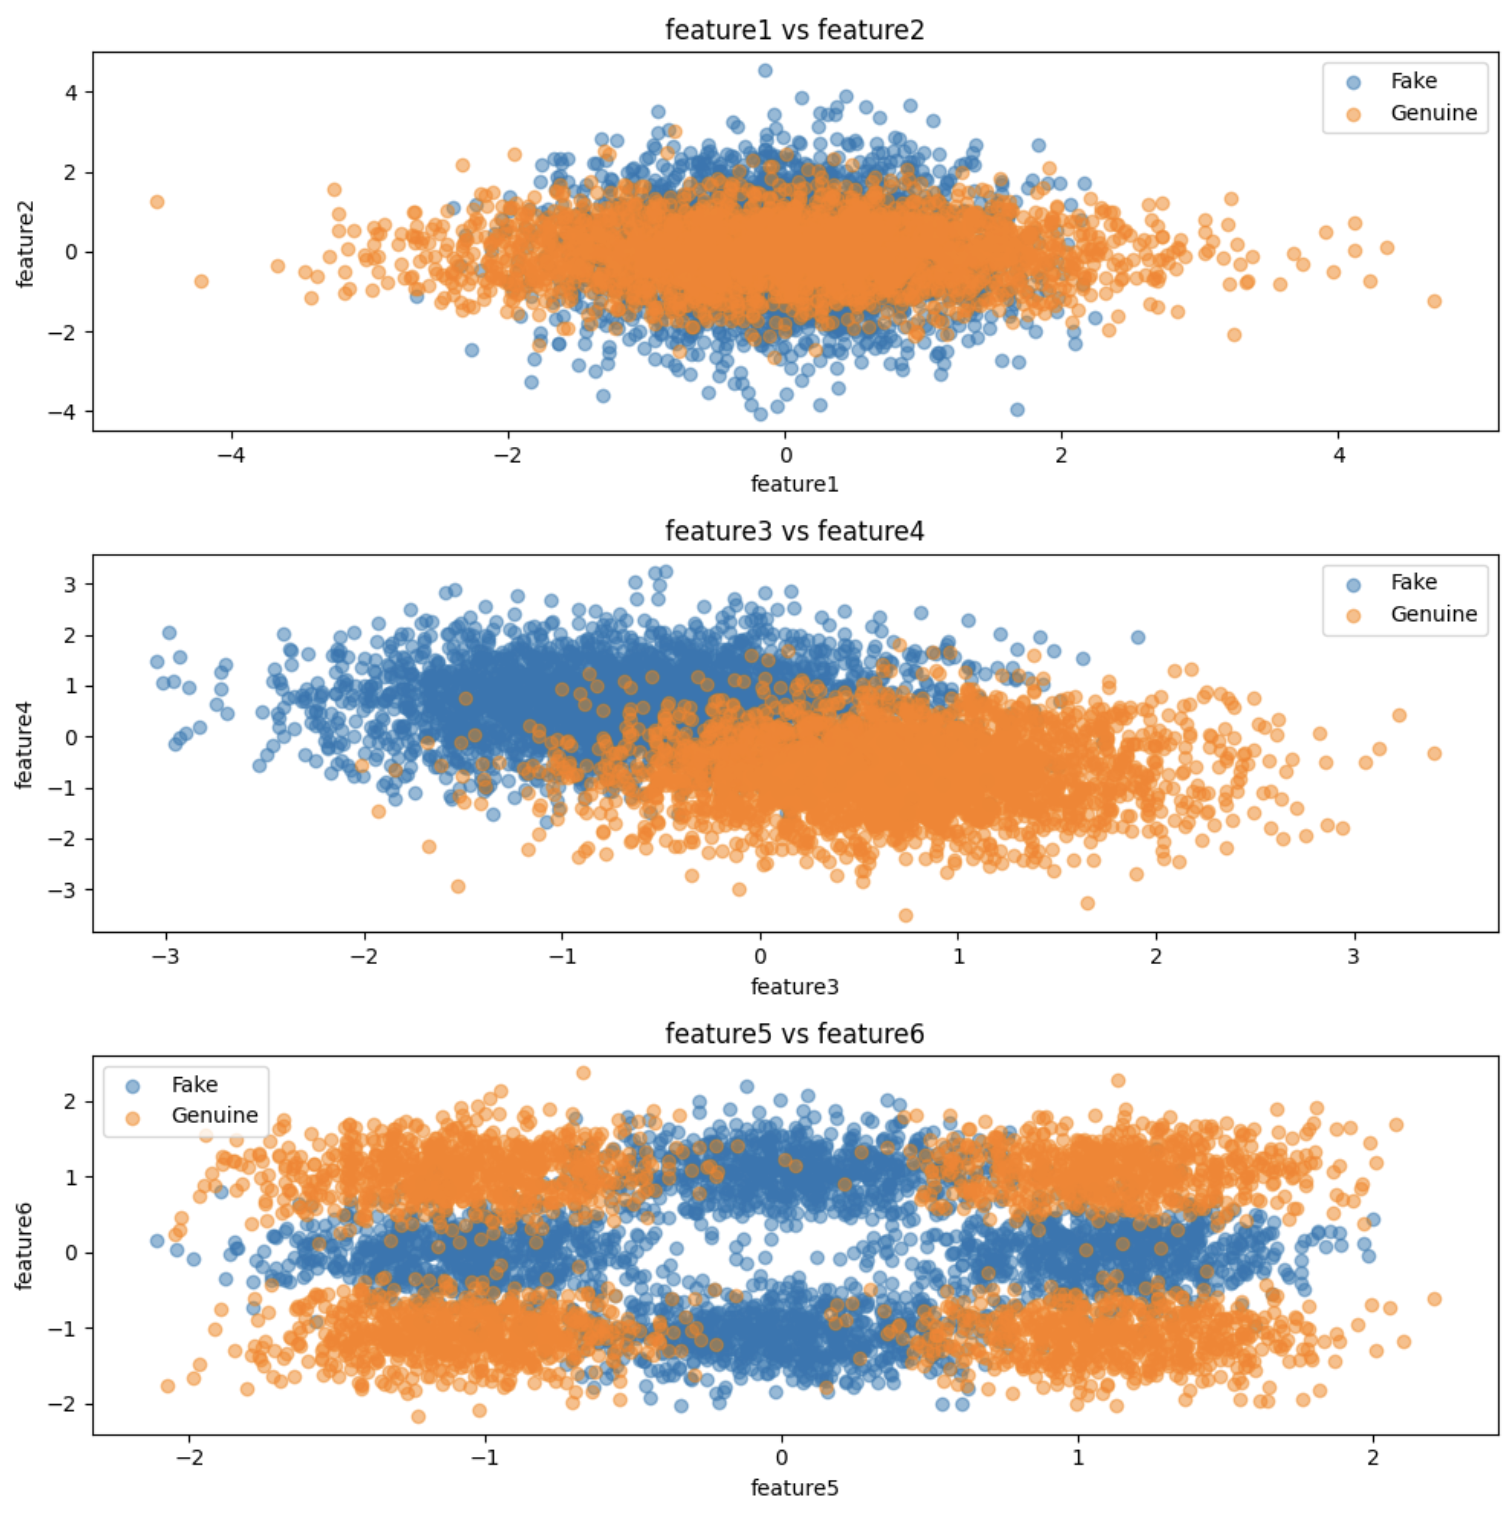
\includegraphics[width=\textwidth]{./img/image2.png}
        \caption{Distribution of feature pairs}
        \label{fig:PairFeatures}
    \end{minipage}
    \hfill % Aggiunge uno spazio orizzontale tra le due minipage se necessario
    \begin{minipage}[b]{0.45\textwidth}
        \centering
        \begin{tabular}{ccc}
            \hline
            Feature & Media & Varianza \\ \hline
            1 & 0.00170711 & 1.00134304 \\
            2 & 0.00503903 & 0.9983527 \\
            3 & -0.00560753 & 1.0024818 \\
            4 & 0.00109537 & 0.99029389\\
            5 & -0.00700025 & 1.00119747 \\
            6 & 0.00910515 & 0.99722374 \\ \hline
        \end{tabular}
        \caption{Mean and variance for each features}
        \label{tab:mean-variance}
    \end{minipage}
\end{figure}
    \\
After making these calculations we can conclude that the data are already centered since all features have mean close to zero.\\
Analyzing the pairwise averages and variances of the features, we can make some observations:  
\begin{itemize}
    \item Feature 1 and Feature 2: These two features have averages very close to zero, indicating that their values are similarly distributed around zero. However, the variance of Feature 2 is slightly lower than that of Feature 1, indicating that the values of Feature 2 are slightly less dispersed than those of Feature 1.  
    \item Feature 3 and Feature 4: Feature 3 has a negative mean, while Feature 4 has a positive mean. This might indicate that the values of Feature 3 tend to be lower than those of Feature 4. Also, the variance of Feature 3 is slightly higher than that of Feature 4, indicating that the values of Feature 3 are more dispersed than those of Feature 4.  
    \item Feature 5 and Feature 6: Feature 5 has a negative mean, while Feature 6 has a positive mean. This might indicate that the values of Feature 5 tend to be lower than those of Feature 6. Also, the variance of Feature 5 is slightly higher than that of Feature 6, indicating that the values of Feature 5 are more dispersed than those of Feature 6. 
\end{itemize}

\section{Dimensionality reduction}
\subsection{PCA}
\subsection{LDA}
\section{Multivariate Gaussian Density}

\section{Classification model analysis}
\subsection{Gaussian Models}
\subsubsection{MVG Gaussian Classifier}
\subsubsection{Naive Bayes Classifier}
\subsubsection{Tied Bayes Classifier}
\subsubsection{Gaussian Models Comparison}
\subsection{Logistic Regression Classifier}
\subsubsection{Quadratic Logistic Regression(QLR)}
\subsection{SVM Classifier}
\subsubsection{Linear SVM}
\subsubsection{Kernel SVM}
\subsection{GMM Classifier}
\section{Score Calibration}
\subsection{Calibration Analysis on Selected Models}
\subsection{Calibrating Scores for Selected Models}
\section{Experimental Results}
\subsection{Calibration on evaluation score}
\subsection{Considerations}
\section{Conclusions}


\newpage



% ------------------------------------------------------------------------------

\end{document}
